\chapter{Introduction}
~~~~~~Although the Higgs boson has been found in 2012 by CMS and ATLAS collaboration~\cite{higgs}, there are no clues of new physics in last running with 3.5 TeV per beam.
the Standard Model still remains many unsolved problems such as neutrino oscillation, the lack of dark matter candidate, fine-tuning and matter anti-matter asymmetry.
On the other hand, it is known that the quarks and neutrinos are mixing as the Cabibbo-Kobayashi-Maskawa (CKM) matrix and Pontecorvo-Maki-Nakagawa-Sakata (PMNS) matrix, respectively~\cite{mark}.
However, as the same family with neutrino, it is strange that charged lepton flavor violation (cFLV) is still not found.
As the prediction of lower branching ratio from the physics beyond the Standard model (BSM), new physics is possible to be probed through the cLFV.

Coherent muon to electron transition (COMET) experiment is planning to seek the cLFV channel of $\mu^- N \rightarrow e^- N$ from 2017.
To achieve the better sensitivity, the most intense muon beamline in J-PARC is under designing and construction.

\section{Charged lepton flavor violation}
~~~~~~In Standard Model, the neutrino oscillation is constricted and massless, in addition, the lepton number is totally conserved when they decay, like
\begin{eqnarray*}
 & \mu^- & \rightarrow  e^-  +  v_\mu  +  \bar v_e  \\
 L_\mu: & 1 & \quad\; 0 \qquad 1 \qquad\! 0 \\
 L_e: & 0 &   \quad\; 1 \qquad 0 \quad -1 
\end{eqnarray*}
where the electron lepton number $L_e$ and muon lepton number $L_\mu$ on left side is conserved on right side.
This decay is the ordinary muon decay and also called Michel decay.
However this is not the only decay for muon, all kinds of muon decay is listed in table~\ref{mudecay}~\cite{pdg}.

Unlike to the michel decay, decay mode of charged lepton like $\mu^- \rightarrow e^- \gamma$ has very tiny probability of decay, observely, its electron and muon lepton number are not conserved on two sides.
The branching ratio predicted by standard model is less than 10$^{-54}$, which the details are described in Appendix.
Otherwise, the physics beyond the standard model such as SUSY-Seasaw, SUSY-GUT etc. predicts the branching ratio higher than 10$^{-15}$, which is possible to be obversed.
The reaction like this is called charged lepton flavor violation.
\begin{table}[H]
 \centering
 \begin{tabular}{cccc} \hline \hline
  Decay modes & Fraction ($\Gamma_i/\Gamma$) & Confidence level & Reference \\ \hline
  $\mu^- \rightarrow e^- \bar\nu_e \nu_\mu$ & $\approx$100 \% & & \\
  $\mu^- \rightarrow e^- \bar\nu_e \nu_\mu \gamma$ & 1.4$_{\pm 0.4}$ \% &  & \cite{critt} \\
  $\mu^- \rightarrow e^- \bar\nu_e \nu_\mu e^+ e^-$ & 3.4$_{\pm 0.4}\times$10$^{-5}$ & &  \\ \hline
  Flavor violating modes & & & \\ \hline
  $\mu^- \rightarrow e^- \nu_e \bar\nu_\mu$ & \textless 1.2 \% & 90 \% & \cite{free} \\
  $\mu^- \rightarrow e^- \gamma$ & \textless 2.4$\times$10$^{-12}$ & 90 \% & \cite{bolton} \\
  $\mu^- \rightarrow e^- e^+ e^-$ & \textless 1.0$\times$10$^{-12}$ & 90 \% & \cite{bertl} \\
  $\mu^- \rightarrow e^- \gamma \gamma$ & \textless 7.2$\times$10$^{-11}$ & 90 \% & \\ \hline \hline
 \end{tabular}
 \caption{Decay modes and branching ratio of muon.}
 \label{mudecay}
\end{table}


\section{Searches for cLFV with muon}
~~~~~$\mu \rightarrow e\gamma$, $\mu \rightarrow eee$ and $\mu \rightarrow e$ conversion are three main decay modes for cFLV seeking, and each mode has its different view in $\mu \rightarrow e$ transition.
In these modes, $\mu \rightarrow e\gamma$ and $\mu \rightarrow eee$ belong to a dipole-type like interaction, however, $\mu \rightarrow e$ conversion is a four-fermion like interaction.
The effective Lagrangian which includes both dipole-type and four-fermion operators is given by~\cite{degou}.
\begin{equation}
 \mathcal{L} = \frac{1}{1+\kappa}\frac{m_\mu}{\Lambda^2}\bar{\mu}_R\sigma^{\mu\nu}e_LF_{\mu\nu} + \frac{\kappa}{1+\kappa}\frac{1}{\Lambda^2}(\bar\mu_L\gamma^\mu e_L)(\bar q_L\gamma_\mu q_L)
 \label{phtoeq}
\end{equation}
%\begin{figure}[H]
% \centering
% 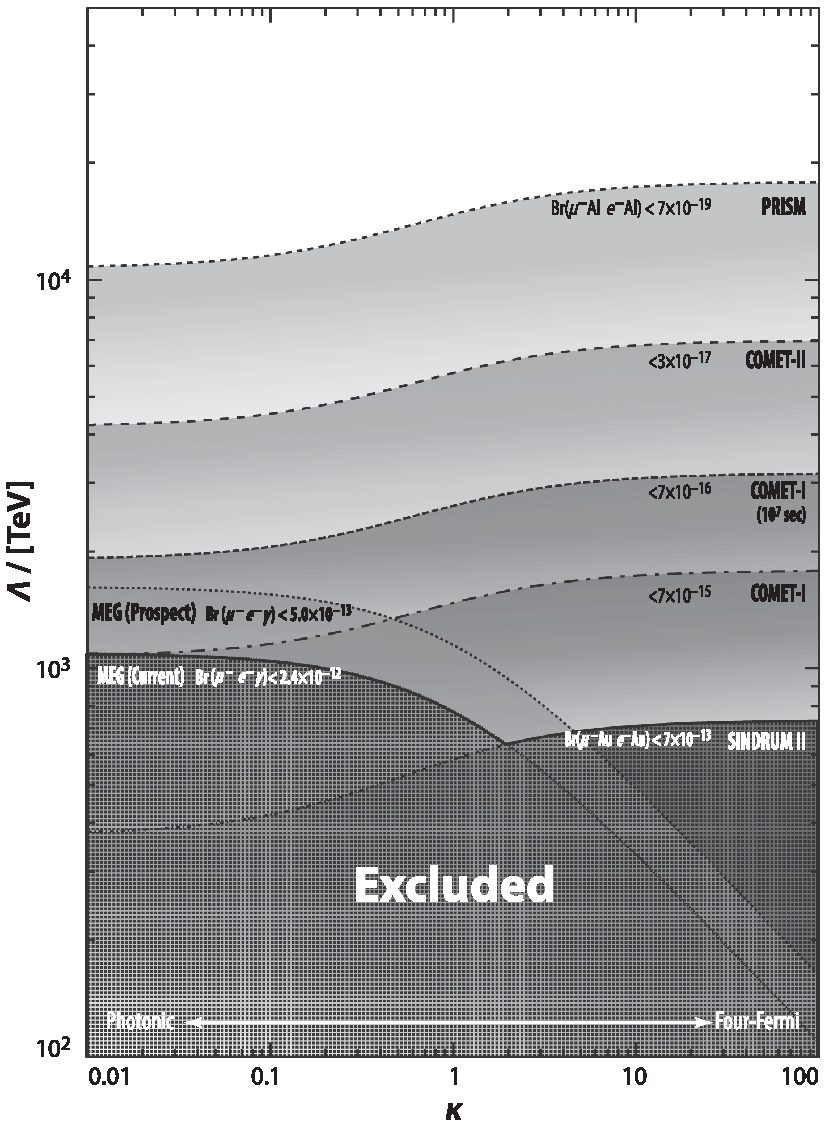
\includegraphics[scale=0.45]{chapter1/fig/photonic.pdf}
% \caption{\it Relation between dipole-like and four-fermion contribution in cLFV.}
% \label{photonic}
%\end{figure}
where $\kappa$ is a parameter which governs the relative size of dipole-type and four-fermion operators.
Parameter $\Lambda$ represents the effective mass (energy) scale of new physics.
The first and second term of this equation are meant to the dipole-like ($\kappa \ll 1$) and four-fermion interaction ($\kappa \gg 1$), which correspond to $\mu \rightarrow e\gamma$ and $\mu \rightarrow e$ conversion, respectively.
%As the result of equation~\ref{phtoeq} shown in figure~\ref{photonic}, the energy scale of new physics is possible to be explored in the TeV range, which exceeds to the range of LHC.

\subsection{$\mu \rightarrow e \gamma$}
~~~~~$\mu \rightarrow e\gamma$ is a 2-body back-to-back decay with monoenergetic $e$ and $\gamma$.
The way to search this decay is to reconstruct these back-to-back monoenergetic $e$ and $\gamma$.
The earliest $\mu \rightarrow e\gamma$ search dates back to 1947 with branching ratio of 0.1 (90\% C.L.)~\cite{1947}, and the most recent experiment for seeking this mode is the MEG experiment.

MEG experiment searches the $\mu^+ \rightarrow e^{+}\gamma$ in Paul Scherrer Institute (PSI) with 3$\times$10$^7$ $\mu^+/sec$.
The data is taken from 2009 to 2010, and MEG experiment is now under upgrading to the phase-II experiment.
As the result, MEG collaboration presents a new upper limit on the branching ratio of this decay of 5.7$\times$10$^{-13}$ (90\% C.L.) with 3.6$\times$10$^{14}$ stopped muons on target~\cite{meg}.

Unfortunately, with the branching ratio of 5.7$\times$10$^{-13}$, there is no signal of interest found finally.
The MEG-II experiment will start data-taking from 2016 to 2019 with 180 days per year and aim to reach the branching ratio of 6$\times$10$^{-14}$~\cite{megtdr}.

\subsection{$\mu \rightarrow eee$}
~~~~~The first experiment for searching $\mu \rightarrow eee$ decay is taken in 1958 at Nevis cyclotron with the branching ratio of 3.0$\times$10$^{-5}$~\cite{lyn}.
Recent best branching ratio is 10$^{-12}$ which is measured by SINDRUM-I experiment.
A new experiment called Mu3e purposes to start from 2016 to reach a branching ratio of $\textless$ 10$^{-16}$ with the requirement of muon stop rate of about 2$\times$10$^9$ $\mu^+$/sec.
Mu3e has two phases, which phase-I and phase-II will taken in $\pi$E5 beamline and HiMB beamline of PSI respectively.

Unlike to $\mu \rightarrow e\gamma$ decay, $\mu^+ \rightarrow e^+e^+e^-$ is a 3-body decay.
The reconstruction of signal of positron and electron must be from the same vertex.
Thus, the challenges of Mu3e are the vertex, timing and momentum resolution~\cite{mu3e}.

\subsection{$\mu \rightarrow e$ conversion}
~~~~~$\mu \rightarrow e$ conversion is a different process from the other two, because the processes of $\mu \rightarrow e\gamma$ and $\mu \rightarrow eee$ are detector-limited owing to accidental background, whilst, the $\mu \rightarrow e$ conversion has no accident background but the background from beam, which depends on the beam qualities.
The past experiments for searching $\mu^- \rightarrow e^-$ conversion is listed in table~\ref{muehis}.
\begin{table}[H]
 \centering
 \begin{tabular}{cccc} \hline \hline
  Target & Upper limit & Place/Collaboration & Year \\ \hline
  Cu & $\textless$ 1.6$\times$10$^{-8}$ & SREL & 1972 \\
  $^{32}$S & $\textless$ 7$\times$10$^{-11}$ & SIN & 1982 \\
  Ti & $\textless$ 1.6$\times$10$^{-11}$ & TRIUMF & 1985 \\
  Ti & $\textless$ 4.6$\times$10$^{-12}$ & TRIUMF & 1988 \\
  Pb & $\textless$ 4.9$\times$10$^{-10}$ & TRIUMF & 1988 \\
  Ti & $\textless$ 4.3$\times$10$^{-12}$ & PSI/SINDRUM II & 1993 \\
  Pb & $\textless$ 4.6$\times$10$^{-11}$ & PSI/SINDRUM II & 1996 \\
  Ti & $\textless$ 6.1$\times$10$^{-13}$ & PSI/SINDRUM II & 1998 \\
  Au & $\textless$ 7$\times$10$^{-13}$ & PSI/SINDRUM II & 2006 \\ \hline \hline
 \end{tabular}
 \caption{History of $\mu^- \rightarrow e^-$ conversion experiments.}
 \label{muehis}
\end{table}
The most precision branching ratio is measured by SINDRUM-II experiment with gold target at PSI.
As shown in figure~\ref{sind}, there is one event found at high momentum region, but it just outside the region of interest.
\begin{figure}[H]
 \centering
 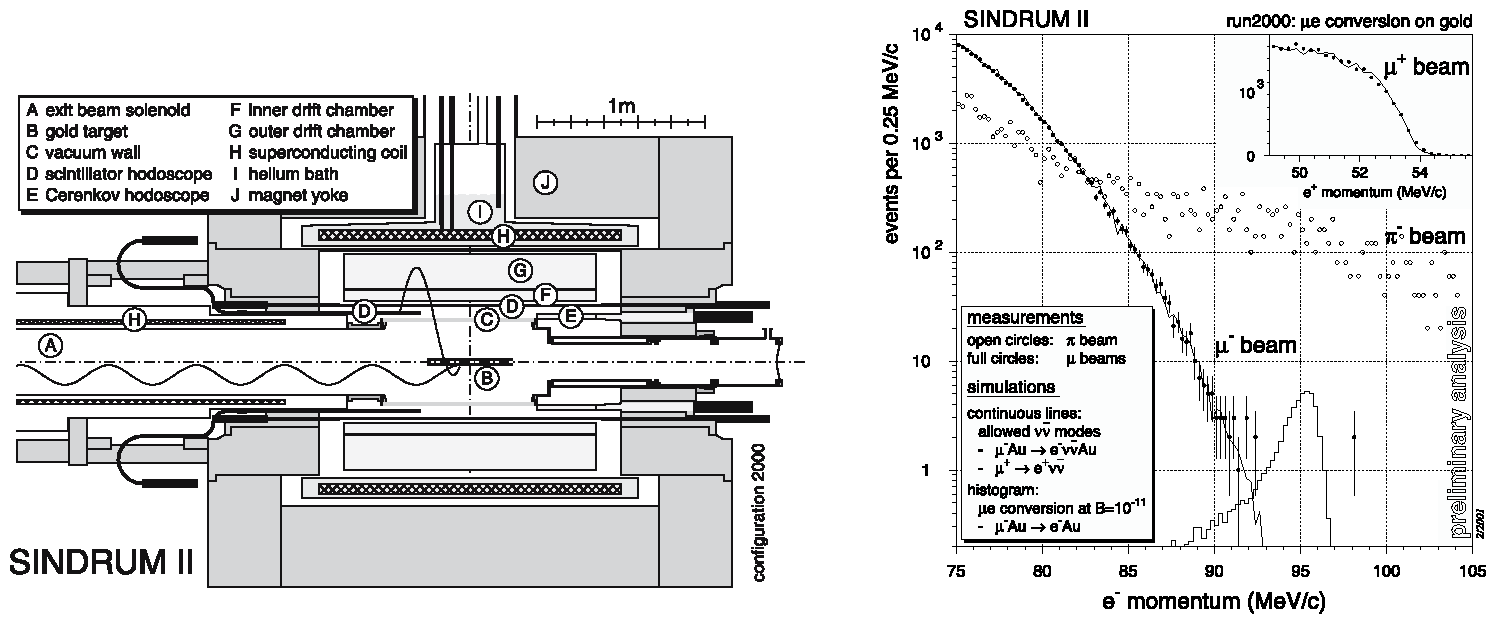
\includegraphics[scale=0.5]{chapter1/fig/sindrum.pdf}
 \caption{SINDRUM-II experiment observes a $\mu^- + Ti \rightarrow e^- + Ti$ conversion with branching ratio of 7$\times$10$^{-13}$. Two signal is found in high energy region but it is out of the range of $\mu^- \rightarrow e^-$ signal.}
 \label{sind}
\end{figure}
COMET and Mu2e experiment are aiming to achieve the branching ratio less than 10$^{-17}$, which is 4 orders less than the previous experimental result.

\section{COMET experiment}
~~~~~~The COMET experiment is designed to search the following $\mu \rightarrow e$ conversion and be carried out at J-PARC.
\begin{equation}
 \mu^- + N(A, Z) \rightarrow e^- + N(A, Z)
\end{equation}
It has two steps for serching cLFV, which are phase-I and phase-II.
phase-I experiment is to measure the background and search for cLFV because the $\mu \rightarrow e$ conversion totally depends on the beam qualities.
phase-II experiment is to seach the $\mu \rightarrow e$ conversion with the sensitivity of 3$\times$10$^{-17}$.
As shown in figure~\ref{comet}, 8 GeV proton hits the target to produce pions, then these pions are captured by magnetic field and transported to the stopping target to generate the signal of $\mu \rightarrow e$ conversion.
The background measurement is taken at the end of 90 degree bending.

To achieve the experimental sensitivity of 3$\times$10$^{-17}$ which corresponds to the branching ratio, a total 2$\times$10$^{18}$ muons stopped in stopping target is needed.
Thus, the high intense muon source with about 10$^{11}$ $\mu^-$/sec is required for COMET experiment.
As for COMET experiment, one COMET dedicated beamline is under construction in J-PARC.
\begin{figure}[H]
 \centering
 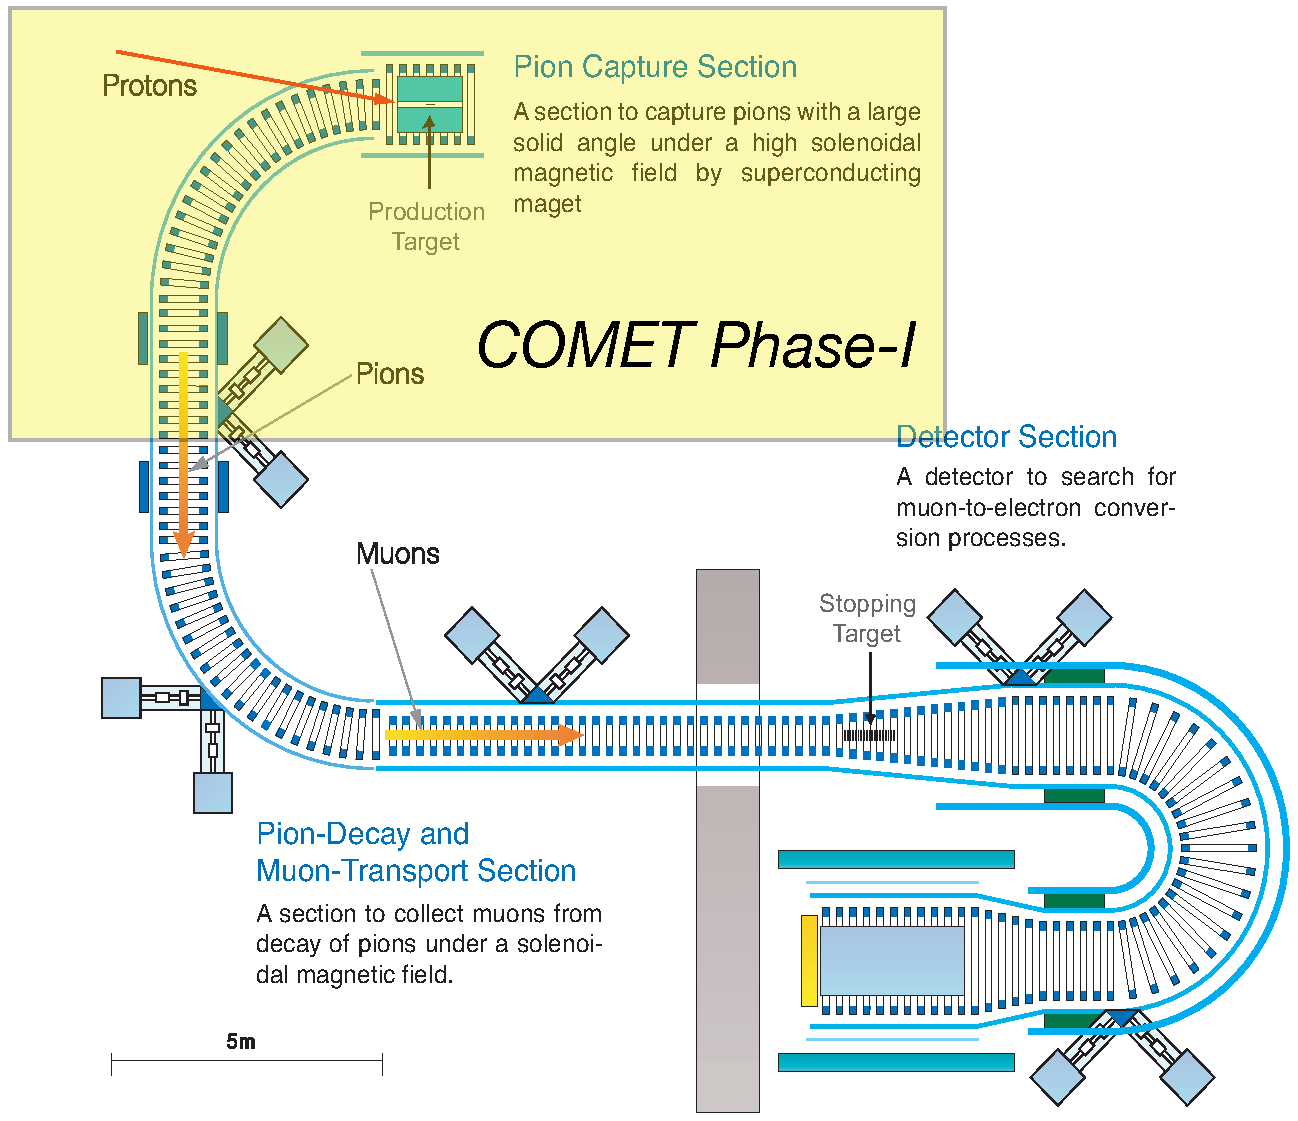
\includegraphics[scale=0.55]{chapter1/fig/comet.pdf}
 \caption{A schematic layout of COMET. 8 GeV proton from B-line hits the target and produce pion first, these pions are captured by pion capture solenoid, and decays to muons in muon transport solenoid. Then, the muon with low momentum is captured by stopping target, meanwhile, an electron with 105 MeV/c from $\mu \rightarrow e$ conversion will be transported to E-cal to take a measurement by detector solenoid.}
\label{comet}
\end{figure}

\subsection{Proton beamline}
~~~~~~To obtain the more precision branching ratio of $\mu \rightarrow e$ conversion, more stopped muon is required.
Stopped muon can be gained from two ways, increasing the operating time and increasing the muon beam intensity.
Since the most intense muon beamline over the world is located in PSI, and it only provides the muon with 4$\times$10$^8$, a new high intense muon beamline is necessary for future particle physics.
Table~\ref{protonbeam} lists the current and future muon beamline, apparently, COMET muon beamline will be the most intense muon beamline over the world in future.
\begin{table}[H]
 \centering
 \begin{tabular}{llll} \hline \hline
 Lab/Beamline & Energy and power & Present $\mu$ rate [Hz] & Future $\mu$ rate [Hz] \\ \hline
 \textbf{PSI:} & & & \\
 LEMS & 590 MeV, 1.3 MW, DC & 4$\times$10$^8$ & \\
 $\pi$E5 & 590 MeV, 1.3 MW, DC & 1.6$\times$10$^8$ & \\
 HiMB & 590 MeV, 1 MW, DC & & 4$\times$10$^{10}$ ($\mu^+$) \\ \hline
 \textbf{J-PARC:} & & & \\
 MUSE D-line & 3 GeV, 1 MW, Pulsed & 3$\times$10$^7$ & \\
 MUSE U-line & 3 GeV, 1 MW, Pulsed & & 4$\times$10$^8$ ($\mu^+$) \\
 COMET & 8 GeV, 56 kW, Pulsed & & $\textgreater$ 10$^{11}$ ($\mu^-$) \\ \hline
 \textbf{FNAL:} & & & \\
 Mu2e & 8 GeV, 25 kW, Pulsed & & 5$\times$10$^{10}$ ($\mu^-$) \\ \hline
 \textbf{TRIUMF:} & & & \\
 M20 & 500 MeV, 75 kW, DC & 2$\times$10$^6$ & \\ \hline
 \textbf{KEK:} & & & \\
 Dai Omega & 500 MeV, 2.5 kW, Pulsed & 4$\times$10$^5$ & \\ \hline
 \textbf{RAL-ISIS:} & & & \\
 RIKEN-RAL & 800 MeV, 160 kW, Pulsed & 1.5$\times$10$^6$ & \\ \hline
 \textbf{RCNP:} & & & \\
 MUSIC & 400 MeV, 400 W, Pulsed & 10$^8$ ($\mu^+$) & \\ \hline
 \textbf{DUBNA:} & & & \\
 Phasatron Ch: I-III & 660 MeV, 1.65 kW, Pulsed & 3$\times$10$^4$ & \\ \hline \hline
 \end{tabular}
 \caption{Current running muon beamline around the world. Current most intense muon beamline is in PSI, COMET muon beamline will be 3 orders higher than PSI muon beamline.}
 \label{protonbeam}
\end{table}

\begin{figure}[H]
 \centering
 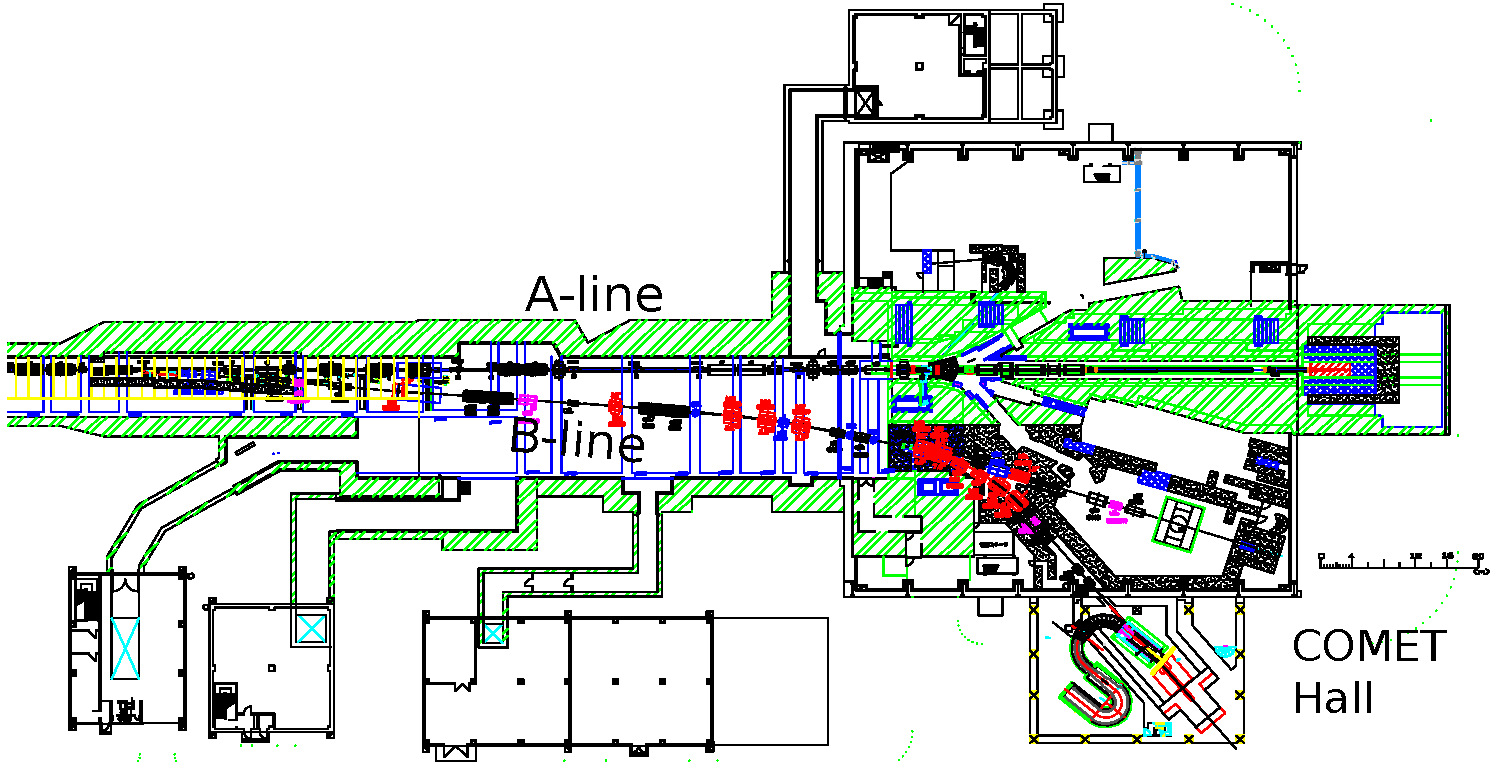
\includegraphics[scale=0.5]{chapter2/fig/beamline.pdf}
 \caption{Dedicated proton beamline for COMET experiment. A new proton beamline, B-line is under construction. COMET Hall is located beside Hadron Hall.}
 \label{bline}
\end{figure}
To accommodate the COMET experiment, a new beamline (B-line) is under construction.
As shown in figure~\ref{bline}, A-line is the existing beamline from the main ring into the Nuclear and Particle Physics (NP) Hall.
B-line is a dedicated proton for COMET experiment.

Both phase-I and phase-II require a pulsed, 8 GeV proton beam slow-extracted from the J-PARC main ring into COMET experimental hall.
The proton beam intensity and production target for phase-I and phase-II is different, which is shown as follows.
In table~\ref{intens}, the requirement of COMET is compared with Mu2e as well.
%Mu2e has a plan to operate for two years to take data, however, COMET only needs 280-day operation to reach the same sensitivity as Mu2e.
\begin{table}[H]
 \centering
 \begin{tabular}{cccccc} \hline \hline
  COMET & Target &  Beam intensity [pps] & Power [kW] & stopped muon [$\mu^-$/sec] & Sensitivity \\ \hline
  phase-I & graphite & 2.5$\times$10$^{12}$ & 3 & 1.30$\times$10$^9$ & 3.1$\times$10$^{-15}$ \\
  phase-II & tungsten & 4.4$\times$10$^{13}$ & 56 & $\textgreater$ 10$^{11}$ & $\textless$3$\times$10$^{-17}$ \\ \hline \hline
%  Mu2e & tungsten & 6$\times$10$^{12}$ & 8 & 2$\times$10$^{10}$ & $\approx$ 10$^{-16}$ \\ \hline \hline
 \end{tabular}
 \caption{Different requirement of proton beam in phase-I and phase-II.}
 \label{intens}
\end{table}


\subsection{Signal of $\mu^-N \rightarrow e^-N$ conversion}
~~~~~~When the $\mu^-N \rightarrow e^-N$ conversion is occurred, the event signal of electron is mono-energetic with energy
\begin{equation}
 E_{\mu e} = m_\mu - B_\mu - E_{rec}
\end{equation}
where $m_\mu$ and $B_\mu$ are mass of muon and bind energy of the 1s monic atom respectively.
$E_{rec}$ is the nuclear recoil energy, which is given by $E_{rec} \approx (m_\mu - B_\mu)^2/2m_N$.
It is very small and can be neglected.
The signal depends on the nuclei, for instance, it is 105.0 MeV for Al stopping target.
This mono-energtic signal is beyond the background, and one tail behind electron background can be observed in $\mu^-N \rightarrow e^-N$ conversion.

Since the muon in aluminum have lifetimes of about 864 nsec, a pulsed proton beam with interval time of 1.17 $\mu$sec is employed to eliminate the prompt background.
As shown in figure~\ref{time}, the prompt background like $\pi^-$ decay is occurred after 100 nsec beyond the proton beam.
Due to the long lifetime of muonic atoms, the time window is opened from 700 nsec to distinguish the background events and signal events.
\begin{figure}[H]
 \centering
 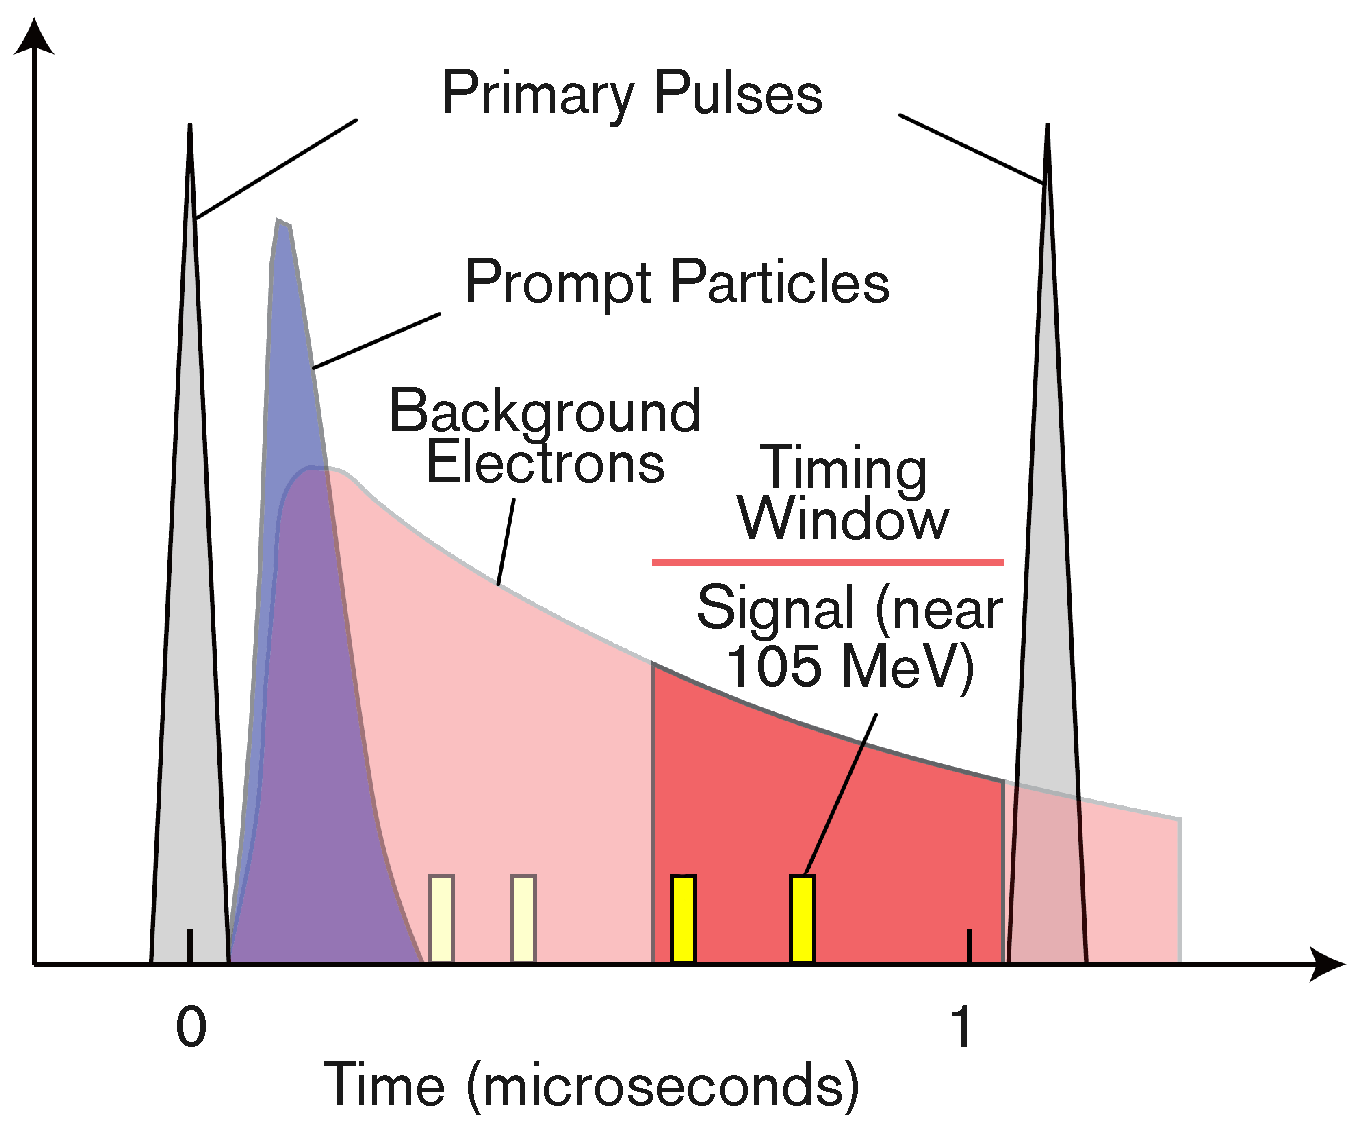
\includegraphics[scale=0.37]{chapter1/fig/time.pdf}
 \caption{The time concept of proton beam. The time window will open from 700 nsec to take data.}
 \label{time}
\end{figure}
The proton beam energy requires a pulsed beam with low production of antiproton and extinction, which will produce the backgrounds.
Therefore, the best choice is 8 GeV for COMET experiment, and the its limit intensity is 4.4$\times$10$^{13}$ pps.
Antiproton can produce the signal like electron and tracked by CDC when it hits the material.
The proton extinction factor is defined as
\begin{equation}
 R_{Ext} = \frac{N_{leak}}{N_{pulse}}
\end{equation}
where $N_{leak}$ is the proton leaked from the pulse, it becomes the background if it comes into the time window, and $N_{pulse}$ is the proton number in the pulse.

\subsection{Background of $\mu^-N \rightarrow e^-N$ conversion}
~~~~~~In COMET experiment, once a $\mu^-$ with low momentum is captured by nuclei, $\mu^-$ will transit to the ground state of 1s.
During this transition, the specific X-ray is emitted from muonic atom.
In addition, the Michel decay in orbit (DIO) emits a electron and dominates the intrinsic background of $\mu \rightarrow e$ conversion.
Without the direct background like DIO, there are many background such as beam related background listed in table~\ref{backg} will cause the indistinguishable signal in CDC during the reconstruction of signal.
\begin{table}[H]
 \centering
 \begin{tabular}{cc} \hline \hline
  Intrinsic physics backgrounds & \\ \hline
  Muon decay in orbit & $\mu^- \rightarrow e^-\nu_\mu\bar\mu_e$ \\
  Radiative muon capture (external) & $\mu^- + A \rightarrow \nu_\mu + A' + \gamma$ \\
  Radiative muon capture (internal) & $\mu^- + A \rightarrow \nu_\mu + A' + e^+ + e^-$ \\
  Neutron emission & $\mu^- + A \rightarrow \nu_\mu + A' + n$ \\
  Charged particle emission & $\mu^- + A \rightarrow \nu_\mu + A' + p (or d or \alpha)$ \\ \hline
  Beam related backgrounds & \\ \hline
  Radiative pion capture (external) & $\pi^- + A \rightarrow \gamma + A', \gamma \rightarrow e^- + e^+$ \\
  Radiative pion capture (internal) & $\pi^- + A \rightarrow e^+ + e^- + A'$ \\
  Beam electrons & $e^-$ scattering \\
  Muon decay in flight & $\mu^-$ decays in flight to produce $e^-$ \\
  Pion decay in flight & $\pi^-$ decays in flight to produce $e^-$ \\
  Neutron induced backgrounds & neutrons hit material to produce $e^-$ \\
  Anti-proton induced backgrounds & anti-proton hit material to produce $e^-$ \\ \hline
  Other background & \\ \hline
  Cosmic-ray induced background & \\
  Room neutron induced background & \\
  False tracking \\ \hline \hline
 \end{tabular}
 \caption{Potential backgrounds for searching $\mu^-N \rightarrow e^-N$ conversion.}
 \label{backg}
\end{table}

\subsubsection{Requirement of magnetic field}
Because the background depends on the muon beam quality, to eliminate the background, the muons must be captured and transported to stopping target efficiently, which can be carried out by using superconducting solenoid magnet system.
The COMET superconsucting magnets must be designed with requirements
\begin{itemize}
 \setlength{\itemsep}{-5pt} 
 \item high magnetic field around the production target to capture the pions.
 \item appropriate magnetic field to transport the low momentum muons to stopping target.
 \item low magnetic field for detector to track the signal electron.
 \item smooth magnetic field to eliminate the trapping of charged particles.
\end{itemize}
The details of magnetic field and superconducting magnet design will be explained in next chapter.

\section{Objetive}
~~~~~~The branching ratio of $\mu^- \rightarrow e^-$ conversion is predicted to around 10$^{-15}$ by the physics beyond the Standard model such as SUSY-GUT, SUSY-Seasaw.
To obtain that experimental sensitivity for searching $\mu^- \rightarrow e^-$ conversion less than 10$^{-17}$, a 8 GeV, 4.4$\times$10$^{13}$ pps proton beam is employed to produce high intense muon beam of 10$^{11}$ $\mu^-$/sec with low momentum.

As the significant part of COMET muon beamline, the pion capture solenoid in superconducting magnet system surrounds a production target with high magnetic field of 5 Tesla and small radius of 672 mm.
Its main issue is the radiation, which cause the over-heat and quench of superconducting magnet due to the thermal conductivity degradation of cooling path and stabilizer.
%which must be designed for working under the high magnetic field and high radiation environment to produce amounts of pion.
%Because the conduction cooling is employed in whole superconducting system, considering the cooling path of superconducting magnets will degrade under high radiation, in this thesis, effects of radiation on superconducting magnet and its radiation resistance have been studied.
Thus, the radiation effects on COMET superconducting solenoid are studied in this thesis.

In chapter 2, the design details of superconducting magnets for COMET phase-I experiment, pion capture solenoid, muon transport solenoid and detector solenoid, will be explained.

In chapter 3, to investigate how much radiation will be produced in COMET experiment, Monte Carlo code is modified to carry out the calculation with COMET condition.
Using the real geometry of COMET experiment, the prompt radiation for phase-II and the residual radiation after phase-I experiment is estimated.
In addition, one radiation shield is designed for protecting the superconducting coils of pion capture solenoid.

In chapter 4, the radiation resistance of the material and device, GFRPs, quench protection diode, insulation tape and pure aluminum, which are used in COMET superconducting magnet system has been tested.

In chapter 5, considering the thermal conductivity will degrade after irradiation, the most important CS1 coils where close to the production target is under risk of quench and over-heat.
Thus, the cooling and quench simulation is estimated.


